\documentclass{article}
\usepackage{../../Self_Style}

\title{Phys 20AL Lab Report Week 3: Pendulum Improvement}
\author{Zih-Yu Hsieh}
\date{\today}

\begin{document}
\maketitle

\tableofcontents

\newpage

\section{Introduction}
As a recall, when calculating the motion of a simple pendulum with arm length $l$, the differential equation describing its motion is $\frac{d^2\theta}{dt^2}=\frac{g}{l}\sin(\theta)$, where $\theta$ denotes the angle of the pendulum. However, this differential equation doesn't have a solution consisting of finite combination / composition of elementary functions (for instance, polynomials, trigonometric functions, exponentials, etc.), which the simpler way of calculating the motion is through approximation.

One common approximation is Small Angle Approximation - which assumes $|\theta|<\epsilon$ for some small enough $\epsilon>0$, so that $\sin(\theta) = \theta+o(\epsilon)$, where $\lim_{\theta\rightarrow 0}\frac{o(\theta)}{\theta}=0$. Then, the differential equation can be approximated as $\frac{d^2\theta}{dt^2}= \frac{g}{l}\theta$, which has a general solution of $\theta(t)=A\cos(\sqrt{\frac{g}{l}}t+\phi)$ for some phase $\phi\in\RR$, and provides the period $\tau = 2\pi\sqrt{\frac{l}{g}}$.

However, such method loses its advantage once the angle of motion becomes large and some nontrivial effect of the pendulum's maximum angle on the period would occur. Hence, the goal of the experiment is to observe such nontrivial effect when angle is no longer considered small.

Beside making the observation, well also verify the validity of the period formula for the non-simplified version (which will be taken up to the degree 4 term):
\begin{align}
    T =2\pi\sqrt{\frac{l}{g}}\left(1+\frac{1}{16}\theta_0^2 + \frac{11}{3072}\theta_0^4.+ ...\right)
\end{align}\label{eq:nontriv}
Here, $T$ is in unit of seconds (s), $g=9.807$ m/s$ ^2$, $l$ is in unit of meters (m), and $\theta_0$ denotes the maximum angle of the pendulum in motion with unit of radians.

\hfil

\section{Experimental Setup (Add image)}
\subsection{Setup with Electronic Detector}
The equipments include: Stand, Clamp, string, spherical mass, protractor, meter stick , detector, and computer.

The following is the steps for setup:
\begin{itemize}
    \item[1.] Setup the stand at the edge of the table.
    \item[2.] Tie one end of the string onto the clamp, pass the other end through the hole at the top of the stand, and clip the clamp onto the stand (to fix the length of the string as pendulum's arm).
    \item[3.] Fix the center of the protractor at the top of the stand at where the pivot of the pendulum is at.
    \item[4.] Fix the spherical mass at the free end of the string (treated as mass of the simple pendulum).
    \item[5.] Fix the detector at the bottom of the stand (the location slightly lower than the spherical mass's position) for ease to detect the period of the spherical mass.
    \item[6.] Connect the detector into the computer for data collection.
\end{itemize}
\begin{figure}[h!]
    \centering
    \begin{subfigure}[t]{0.3\textwidth}
        \centering
        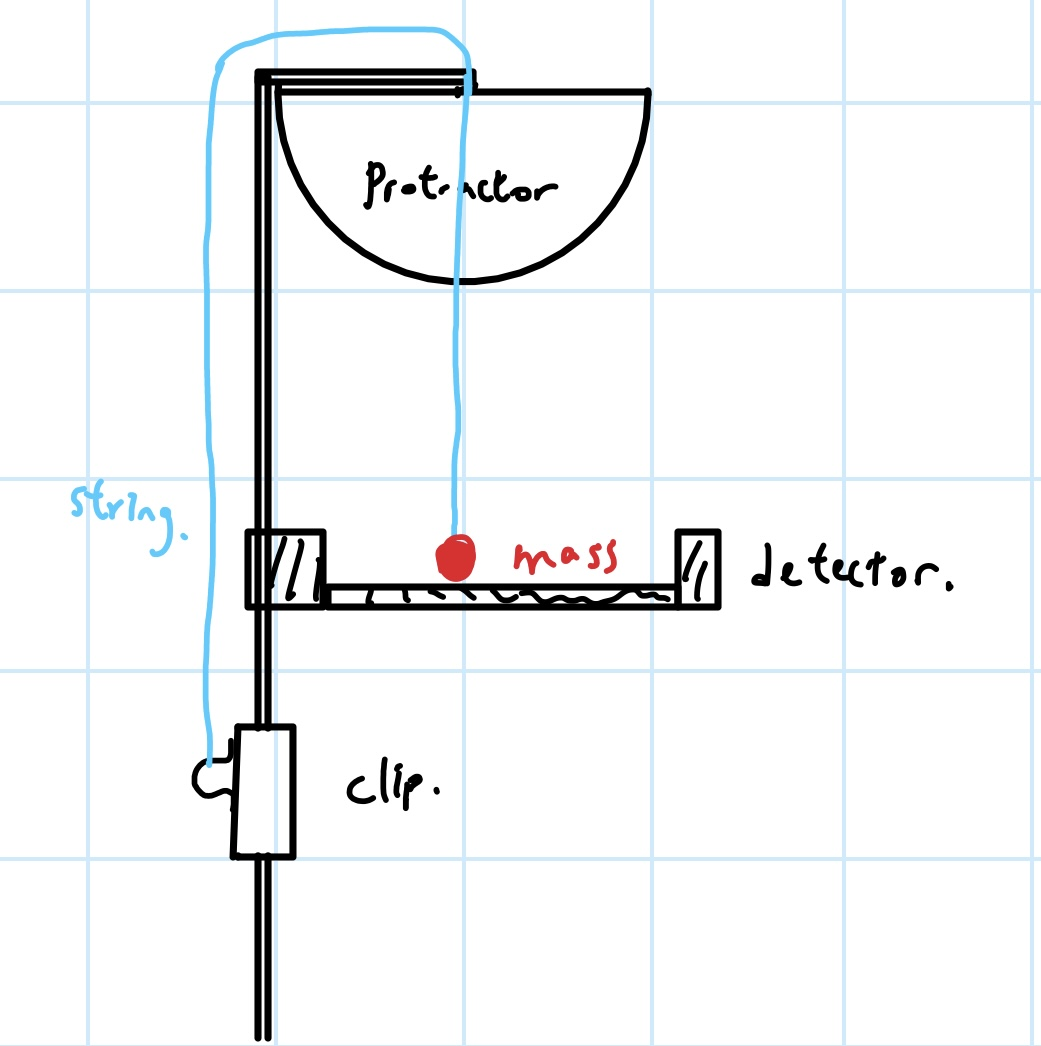
\includegraphics[width=\linewidth]{sketch_detector.jpg}
        \caption{Sketch of the Equipment Setup (With Detector)}
        \label{fig:sketch_setup}
    \end{subfigure}%
    \hfil 
    \begin{subfigure}[t]{0.2\textwidth}
        \centering
        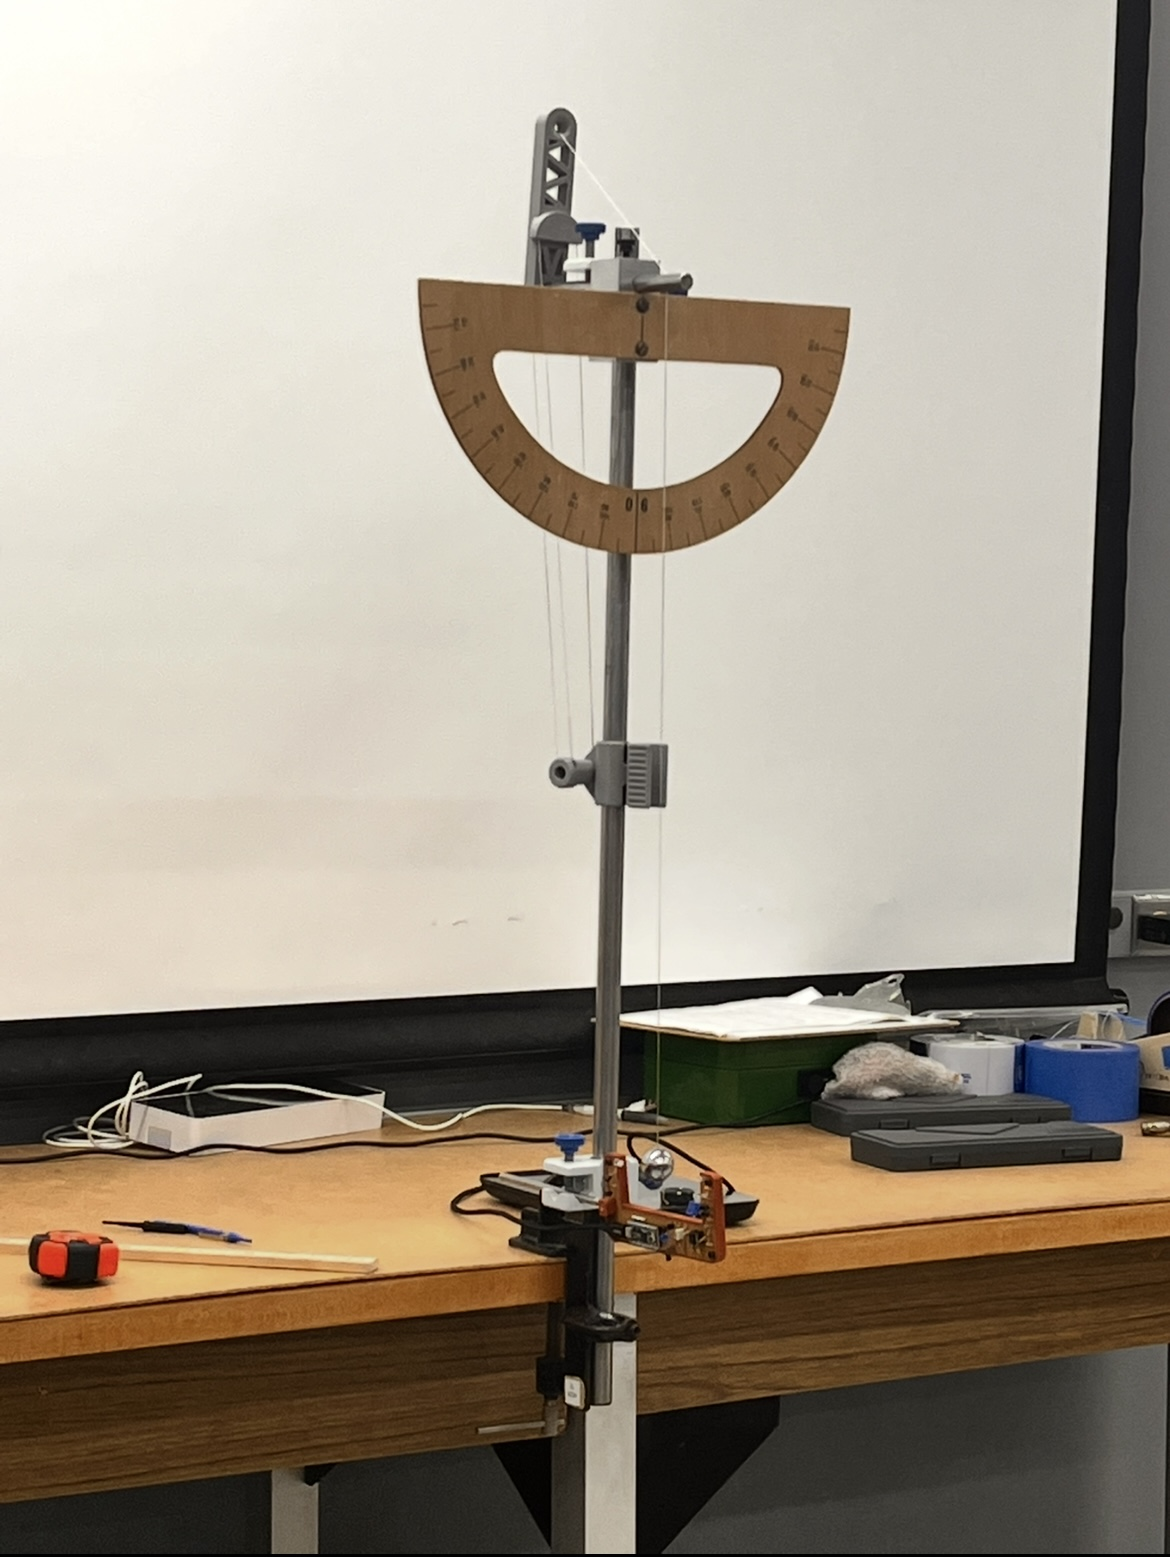
\includegraphics[width=\linewidth]{setup_electronic.jpg}
        \caption{Photo of the Equipment Setup (With Detector)}
        \label{fig:physical_setup}
    \end{subfigure}
\end{figure}

\newpage

\subsection{Setup without Electronic Detector}
Equipments include: Stand, Clamp, string, spherical mass, protractor, meter stick , timer, phone (use as camera).

The setup is nearly identical with the description in \textbf{2.1}, except for not fixing a detector on the stand.
\begin{figure}[h!]
    \centering
    \begin{subfigure}[t]{0.3\textwidth}
        \centering
        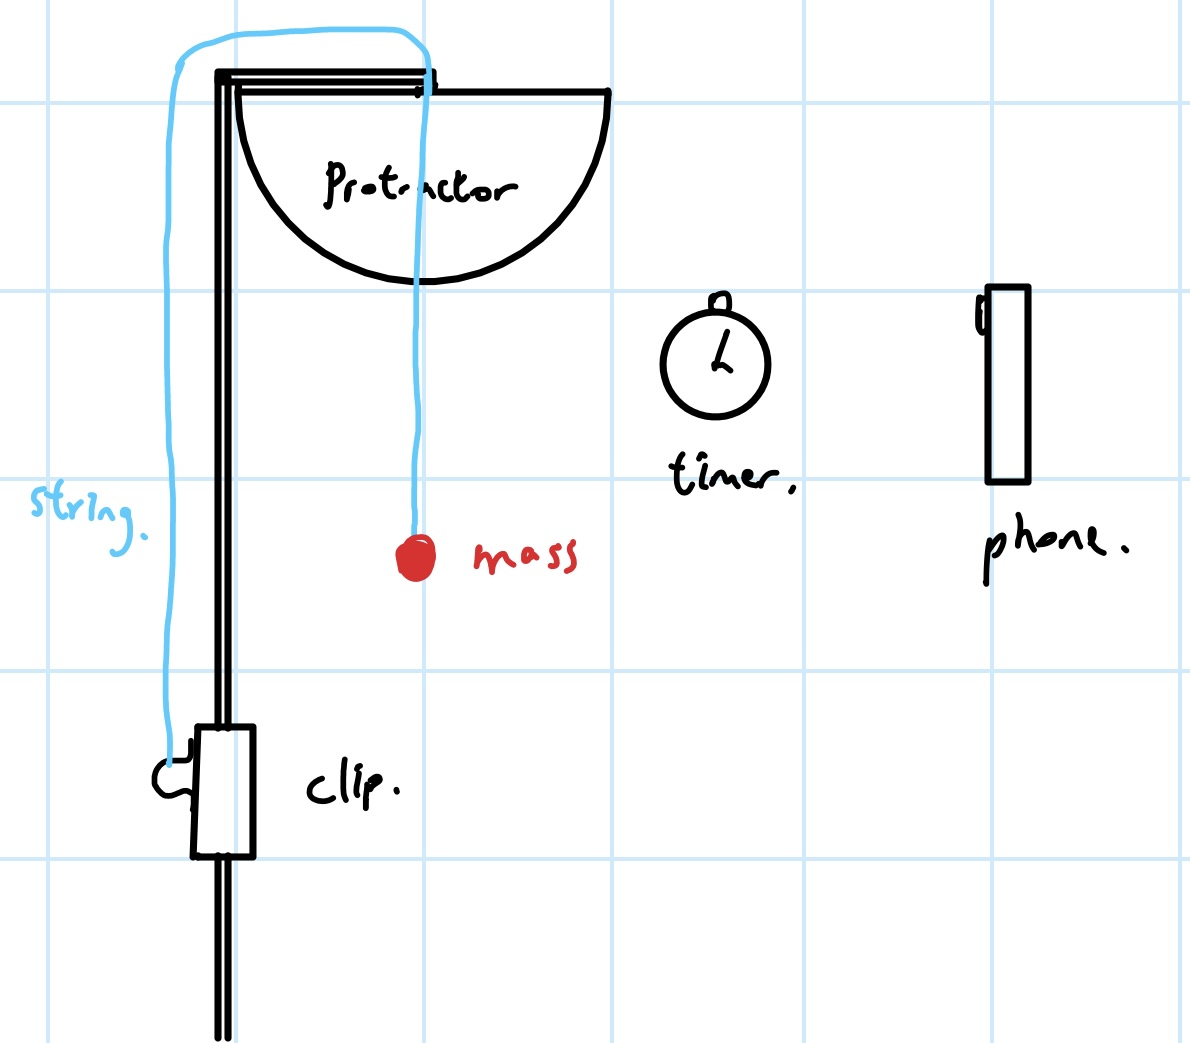
\includegraphics[width=\linewidth]{sketch_no_detector.jpg}
        \caption{Sketch of the Equipment Setup (Without Detector)}
        \label{fig:sketch_setup}
    \end{subfigure}%
    \hfil 
    \begin{subfigure}[t]{0.2\textwidth}
        \centering
        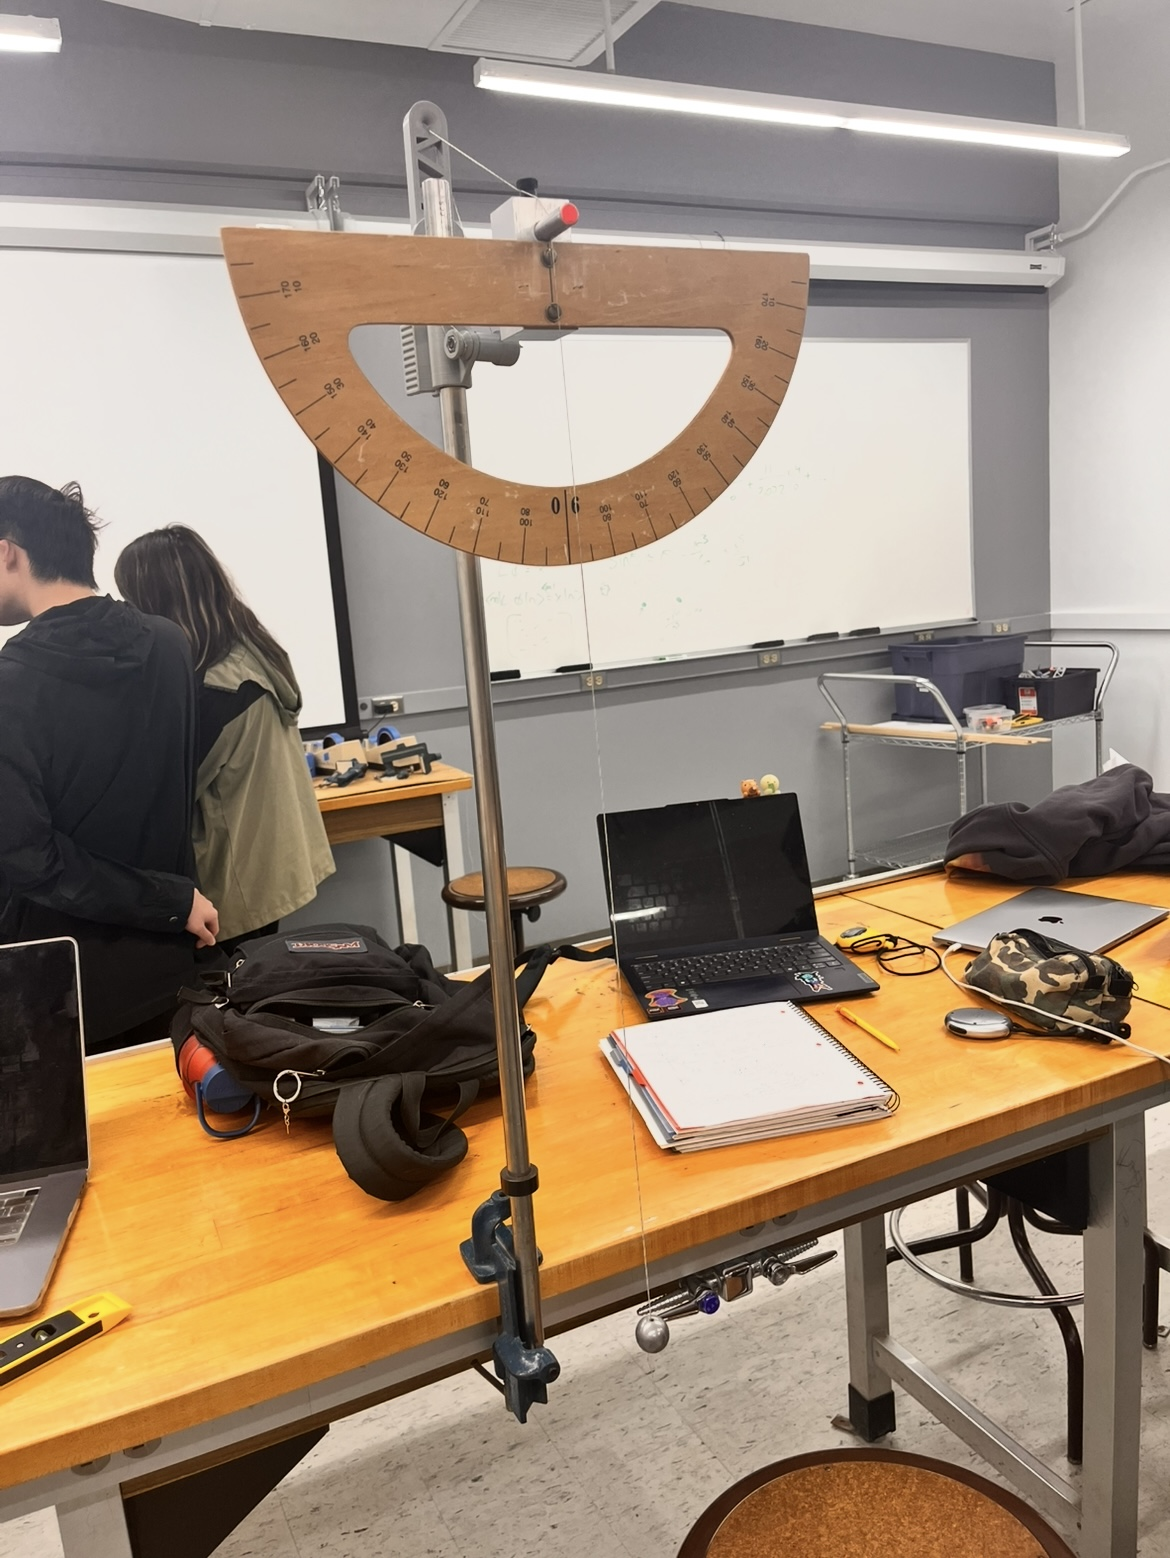
\includegraphics[width=\linewidth]{setup_no_electroinc.jpg}
        \caption{Photo of the Equipment Setup (Without Detector)}
        \label{fig:physical_setup}
    \end{subfigure}
\end{figure}

\newpage


\section{Methods of Measurement and Procedure}
\subsection{What to Measure and Measurement Method}
For each fixed manipulated variable, we'll measure total of $5$ trials.

\hfil

For both experiment, the manipulated variables are the maximum angle of the pendulum (recorded in degrees $ ^\circ$, and measured using protractor). Both experiments used angles $\theta=10^\circ, 20^\circ, 30^\circ, 40^\circ$, and $50^\circ$. 

Also, the mass of the pendulum is measured through mass scale, and fixed as $65$ g (or $0.065$ kg); the length of the pendulum is measured using meter stick, where for the setup with Detector, the fixed length is $65.5$ cm (or $0.655$ m), while the fixed length for the setup without Detector is $75.5$ cm (or $0.755$ m).

\hfil

The responding/dependent variable on the other hand, is the time period of the pendulum under the given angle. In the two setups, the measurements are done differently:
\begin{itemize}
    \item \textbf{Setup with Detector:} The detector records the time when the pendulum passes through the lowest point, which serves as a recording of time period.
    \item \textbf{Setup without Detector:} It involves fixing the timer in the background environment of the pendulum, let the timer runs normally, and use the phone camera to record the whole pendulum motion. Afterward, we'll check individual frames of the recording fo get a more precise measurement of the time period.
\end{itemize}

\subsection{Procedure}
\subsubsection{Setup with Electronic Detector}
We followed the procedure below:
\begin{enumerate}
    \item Turn on the electronic detector and computer for measurement.
    \item Fix an angle to be experimented with, and raise the pendulum to the fixed angle.
    \item Release the pendulum, and let it swing for ten cycles.
    \item Repeat Steps 2 to 3 for total of five trials.
    \item Now, change the angle to other desired values, and repeat Steps 2 to 4 for every desired angle.
\end{enumerate}

\subsubsection{Setup without Electronic Detector}
We followed the procedure below:
\begin{enumerate}
    \item Fix the timer in the background environment (behind the pendulum specifically), and fix the phone / camera in front of the pendulum and the timer (\textbf{Rmk}: Need to ensure the phone can clearly capture the timer value and the motion of the pendulum).
    \item Fix an angle to be experimented with, and raise the pendulum to the fixed angle.
    \item Release the pendulum, and let it swing for five cycles.
    \item Repeat Steps 2 to 3 for total of five trials.
    \item Now, change the angle to other desired values, and repeat Steps 2 to 4 for every desired angle.
\end{enumerate}

\newpage

\section{Experimental Data and Tables}
For the collected data, instead of calculating period of each individual cycle, here it's simplified to an average period of all cycles when the pendulum is in motion.
\subsection{Data with Electronic Detector}
Here, the length of the pendulum is $0.655$ m, for each trial recorded over $10$ pendulum cycles.
\begin{table}[h!]
\centering
\begin{tabular}{c||c|c|c|c|c}
\toprule
\diagbox[width=3cm,height=1cm]{\textbf{Trial}}{\textbf{Angle (°)}} & \textbf{10°} & \textbf{20°} & \textbf{30°} & \textbf{40°} & \textbf{50°} \\
\midrule
1 & 1.633 & 1.639 & 1.653 & 1.676 & 1.698 \\
\hline
2 & 1.633 & 1.639 & 1.652 & 1.677 & 1.696 \\
\hline
3 & 1.633 & 1.639 & 1.653 & 1.677 & 1.694 \\
\midrule
\textbf{Mean} & \textbf{1.633} & \textbf{1.639} & \textbf{1.653} & \textbf{1.676} & \textbf{1.696} \\
\hline
\textbf{SD} & \textbf{0.000} & \textbf{0.000} & \textbf{0.000} & \textbf{0.001} & \textbf{0.002} \\
\bottomrule
\end{tabular}
\caption{Average period (unit: s) of Pendulum under Various Maximum Angles (With Detector)}
\label{tab:data_elect}
\end{table}
\begin{figure}[h!]
    \centering
    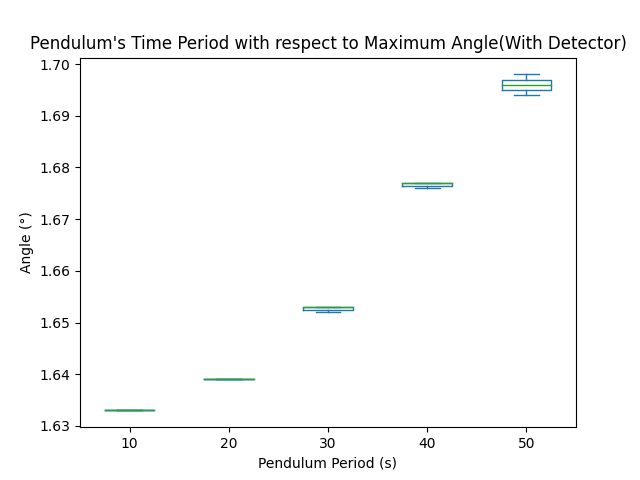
\includegraphics[width=100mm]{1.png}
\end{figure}

The presented data and graph is as expected, since based on the provided formula of (maximum angle dependent) pendulum period in \ref{eq:nontriv}, the the period of the pendulum is increasing when the maximum angle increases, and this is demonstrated in the above graph.

\newpage

\subsection{Data without Electronic Detector}
Here, the length of the pendulum is $0.755$ m, for each trial recorded over $5$ pendulum cycles.
\begin{table}[h!]
\centering
\begin{tabular}{c||c|c|c|c|c}
\toprule
\diagbox[width=3cm,height=1cm]{\textbf{Trial}}{\textbf{Angle (°)}} & \textbf{10°} & \textbf{20°} & \textbf{30°} & \textbf{40°} & \textbf{50°} \\
\midrule
1 & 1.762 & 1.798 & 1.800 & 1.830 & 1.811 \\
\hline
2 & 1.760 & 1.774 & 1.800 & 1.833 & 1.813 \\
\hline
3 & 1.764 & 1.788 & 1.780 & 1.647 & 1.804 \\
\midrule
\textbf{Mean} & \textbf{1.762} & \textbf{1.787} & \textbf{1.793} & \textbf{1.770} & \textbf{1.809} \\
\hline
\textbf{SD} & \textbf{0.002} & \textbf{0.012} & \textbf{0.012} & \textbf{0.107} & \textbf{0.005} \\
\bottomrule
\end{tabular}
\caption{Average period (unit: s) of Pendulum under Various Maximum Angle (No Detector)}
\label{tab:data_no_elect}
\end{table}
\begin{figure}[h!]
    \centering
    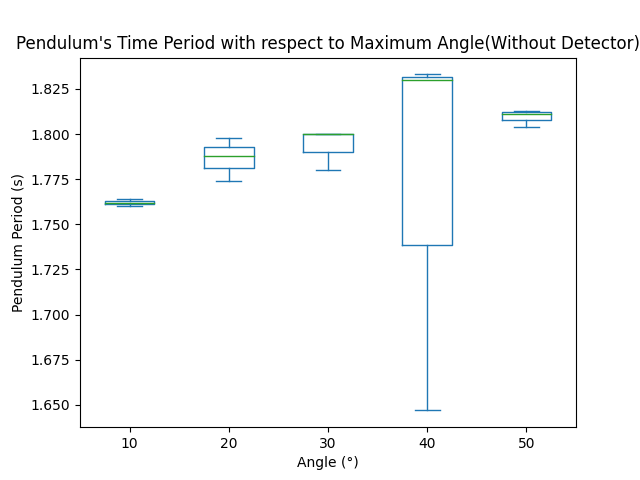
\includegraphics[width=100mm]{2.png}
\end{figure}

The presented data and graph are mostly as expected, except for some parts with larger uncertainty. The trend of the data based on the graph above still demonstrates an increase in pendulum period (in general) when the maximum angle increases. However, for angle of $40$° it is with an unexpectedly high uncertainty, which is not an expected part.

\hfil

\newpage

\section{Data Analysis}
From the data demonstrated in \textbf{Table \ref{tab:data_elect}} and \textbf{\ref{tab:data_no_elect}}, since both set of datas have low uncertainties in comparisan to the mean of the average period (in general, all Standard Deviation is below $0.107$). Hence, it implies the mean of the average pendulum period can serve as a valid representative of the pendulum's period within the experiment.

Here, the \textbf{Expected Period} of the pendulum will be calculated through Formula \ref{eq:nontriv}, while truncating the infinite series to a degree $4$ polynomial.

\subsection{Analysis with Eletronic Detector}
\begin{table}[h!]
\centering
\begin{tabular}{c||c|c|c|c|c}
\toprule
\textbf{Angle (radians)} & 0.028 & 0.029 & 0.029 & 0.029 & 0.030 \\
\hline
\textbf{Mean Average Period (s)} & 1.633 & 1.639 & 1.653 & 1.676 & 1.696 \\
\hline
\textbf{Expected Period (s)} & 1.639 & 1.649 & 1.664 & 1.686 & 1.714 \\
\hline
\textbf{Percent Error (\%)} & 0.384 & 0.587 & 0.679 & 0.604 & 1.083 \\
\bottomrule
\end{tabular}
\caption{Comparison of Mean Average Period (unit: s) and the Expected Period (With Detector)}
\label{tab:compare_elect}
\end{table}

Using the period equation in \ref{eq:nontriv}, the expected pendulum periods are calculated for each angle (in terms of radians). Which, compare the calculation with the mean of Average Period for each angle, each angle yields an extremely low percent error, with the minimum of $0.384\%$ and the maximum of $1.083\%$, showing the collected datas are pretty similar to the expected period calculated by the formula. Hence, the formula in fact has a high validity of representing the relation between maximum angle and the period of a pendulum, in this experiment with Electronic Detector.

\hfil

\subsection{Analysis without Electronic Detector}
\begin{table}[h!]
\centering
\begin{tabular}{c||c|c|c|c|c}
\toprule
\textbf{Angle (radians)} & 0.031 & 0.031 & 0.031 & 0.032 & 0.032 \\
\hline
\textbf{Mean Average Period (s)} & 1.762 & 1.787 & 1.793 & 1.770 & 1.809 \\
\hline
\textbf{Expected Period (s)} & 1.747 & 1.757 & 1.774 & 1.798 & 1.830 \\
\hline
\textbf{Percent Error (\%)} & 0.870 & 1.676 & 1.095 & 1.579 & 1.139 \\
\bottomrule
\end{tabular}
\caption{Comparison of Mean Average Period (unit: s) and the Expected Period (No Detector)}
\label{tab:compare_noelect}
\end{table}

Again, using the period equation in \ref{eq:nontriv}, comparing the calculated expected period with the mean of Average Period for each angle, each angle yields an extremely low percent error, with the minimum of $0.870\%$ and the maximum of $1.676\%$, showing the collected datas are still similar to the expected period calculated by the formula. Hence, the formula still maintains a high validity of representing the relation between maximum angle and the period of a pendulum, in this experiment without Electronic Detector.

\newpage

\section{Error Analysis}
\subsection{Setup with Electronic Detector}
In this experiment, since the time measurement is using electronic detector instead of human perception and timer, some of the potential human measurement mistakes are prevented. The only potential source of human mistake is the maximum angle measurement, which is still relying on human eyes.

Besides the human error, the potential sources of error include:
\begin{itemize}
    \item Air Resistance and Friction, which potentially add in external forces that couldn't be directly observed, dissipating the energy of the system, and decrease the maximum angle at each cycle in between the experiment. 
    \item Electronic Detector's measurement error, which the uncertainty within the electronic detector's measurement couldn't be directly observed by human, and also extremely difficult to verify with the other equipments provided.
\end{itemize}

\hfil

\subsection{Setup without Electronic Detector}
In this experiment, although the time measurement is made (and recorded) by timer and phone camera, but the actual time collection (into the data sheet) are still made by human, through looking at the phone's recording. Which, this provides an extra potential source of human mistake (since checking the video file still relies on human perception about when the pendulum starts and end).

Besides the human mistakes, the potential source of error are identical to the first source of error (about air resistance and friction) described in \textbf{6.2}.

\hfil

\section{Conclusion}
In this lab, the experimental data suggested that there is a high confidence that the pendulum period is provided by $T=2\pi\sqrt{\frac{l}{g}}\left(1+\frac{1}{16}\theta_0^2+\frac{11}{3702}\theta_0^4+..\right)$ (in the Data Analysis it is truncated to a formula with degree $4$), where $\theta_0$ is the pendulum's maximum angle (unit: radians).

The potential sources of error (besides human measurement mistakes) include air resistance and friction, while for the experiment with Electronic Detector, there is an extra potential source of error coming from the detecting device itself.


\end{document}